\section{Introduction}
Segmentation and clustering of large amounts of data is one important research field of artificial intelligence.

In recent years, with the expansion and diffusion of the digitalization of physical archives, both in the private and public sector, these techniques have become increasingly prominent for economic and financial reasons since they can easily shrink the amount of man-hours needed to achieve the tasks involved. 

Related to these circumstances, the application developed in this work presents an approach to group together handwritten words with similar visual shape.
The intent of the application is to make possible the grouping of images, representing the same word, contained in handwritten scanned documents in sets with a predefined minimum precision.
From these sets a human operator can thus categorize all the words through the apposition of a single label per set, rather than per element, with obvious gains in time and costs.

  
The basis of this work is the collection of U.S. Census data of the year 1930.
The goal is to divide enrollees by state: this is done through the clustering of the handwritten words contained in the "State" field of the forms.

Document segmentation and extraction of the words corresponding to the states was developed previously by two of our colleagues in the course of \emph{Technology of Databases} for documents with a structure similar to the one of our dataset.
Their project is thus the starting point of this work: the main contribution of this project to the preexisting work is in the definition of a different, more relevant, valuation method through which determine the distance between different images, in hope that the results may have a greater precision.
The method proposed in this work is based on the use of \textit{structural features}, directly connected to the stroke with which the words were written. 
The main problem on which we have worked is thus the extraction of features from handwritten words with the goal of creating clusters of similar elements so as to facilitate the recognition by a human agent.

\begin{figure}[!ht]
\centering
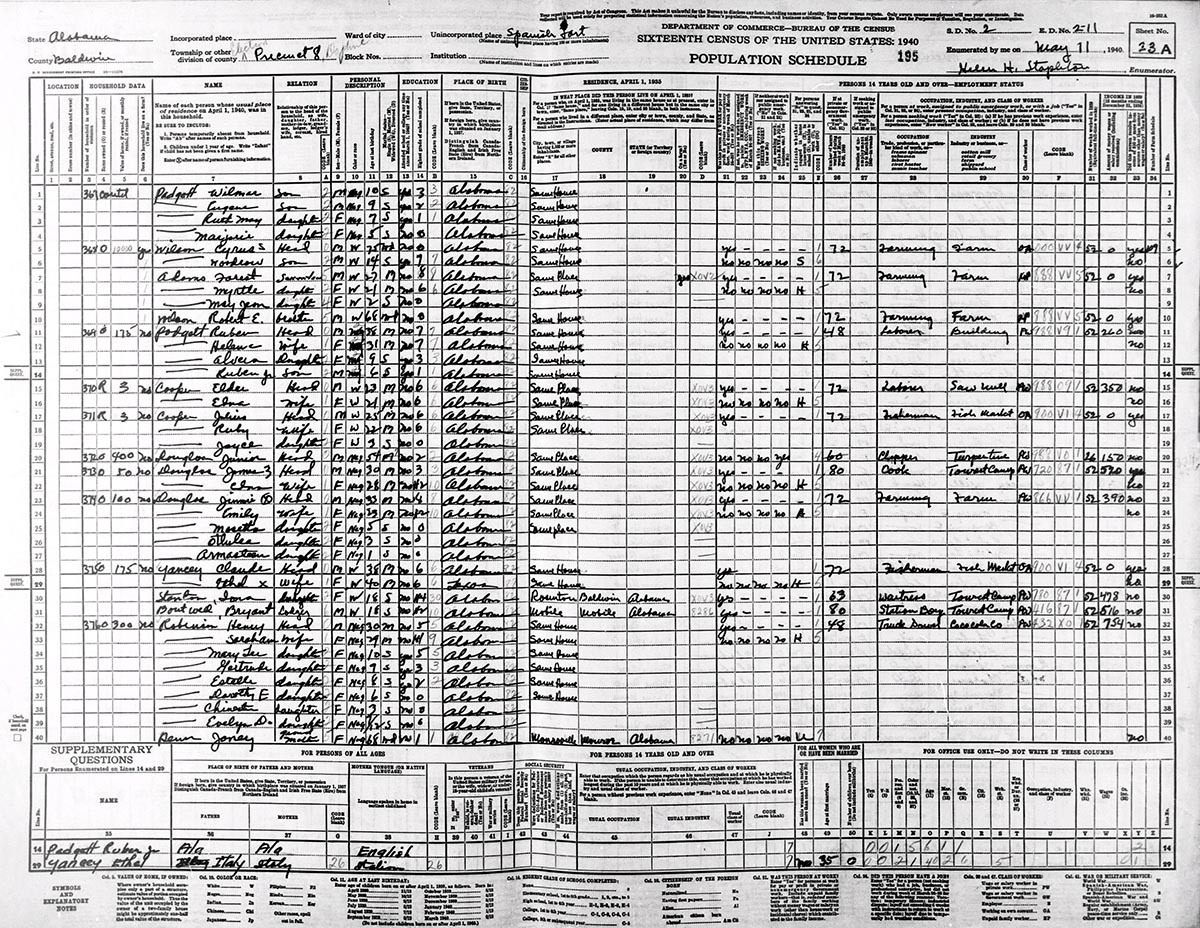
\includegraphics[width=0.66\textwidth]{images/img1.jpg}
\caption{An example of a table containing census data}
\end{figure}